\documentclass[
	a4paper,
	twoside,
	12pt
]{book}

\usepackage{adjustbox}
\usepackage{amsmath}
\usepackage{amsthm}
\usepackage[italian]{babel}
\usepackage[backend=biber, style=ieee, dashed=false]{biblatex}
\usepackage{bm} 
\usepackage{caption}
\usepackage[style=italian]{csquotes}
\usepackage{diagbox}
\usepackage{enumitem}
\usepackage{fancyhdr}
\usepackage[T1]{fontenc}
\usepackage{frontespizio}
\usepackage[top=3cm, bottom=3cm, left=3cm, right=3cm]{geometry}
\usepackage{graphicx}
\usepackage{parskip}
\usepackage{placeins}
\usepackage{setspace}
\usepackage{siunitx} 
\usepackage{todonotes}
\usepackage{xcolor}
\usepackage{xurl}
\usepackage[breaklinks=true,colorlinks=false,linkbordercolor=blue,urlbordercolor=blue,citebordercolor=blue]{hyperref}
\usepackage{listings}

\addbibresource{./Bibliografia/Bibliografia.bib}

\newtheoremstyle{StileEsempio}
  {\topsep}     % Spazio sopra
  {\topsep}     % Spazio sotto
  {\normalfont} % Font del corpo del testo
  {}            % Indentazione
  {\bfseries}   % Font dell'intestazione
  {}            % Indentazione
  {\newline}    % A capo dopo il titolo
  {}            % Specifica dell'intestazione
\theoremstyle{StileEsempio}
\newtheorem{esempio}{Esempio}[chapter]

\graphicspath{{./Immagini}}
\onehalfspacing

\newcommand{\CC}{C\nolinebreak\hspace{-.05em}\raisebox{.4ex}{\tiny\bf +}\nolinebreak\hspace{-.10em}\raisebox{.4ex}{\tiny\bf +}}

\pagestyle{fancy}
\fancyhf{}
\fancyfoot[LE,RO]{\thepage}
\renewcommand{\headrulewidth}{0pt}
\fancypagestyle{plain}{
  \fancyhf{}
  \fancyfoot[LE,RO]{\thepage}
  \renewcommand{\headrulewidth}{0pt}
}

\hyphenation{MATLAB}

\definecolor{codegreen}{rgb}{0,0.6,0}
\definecolor{codegray}{rgb}{0.5,0.5,0.5}
\definecolor{codepurple}{rgb}{0.58,0,0.82}
\definecolor{backcolour}{rgb}{0.95,0.95,0.95}

\lstdefinestyle{MatlabStyle}{
    language=Matlab,
    backgroundcolor=\color{backcolour},   
    commentstyle=\color{codegreen},
    keywordstyle=\color{blue},
    numberstyle=\tiny\color{codegray},
    stringstyle=\color{codepurple},
    basicstyle=\ttfamily\footnotesize,
    breakatwhitespace=false,         
    breaklines=true,                 
    captionpos=b,                    
    keepspaces=true,                 
    numbers=left,                    
    numbersep=5pt,                  
    showspaces=false,                
    showstringspaces=false,
    showtabs=false,                  
    tabsize=2,
    frame=single,
    framerule=0pt,
    framesep=5pt,
    framexleftmargin=2pt
}
\lstset{style=MatlabStyle}

\sisetup{output-decimal-marker = {,}, product-units = single, detect-weight}

\setlength{\parindent}{0pt}
\setlength{\parskip}{1em}
\raggedbottom

\begin{document}
%Inizio Introduzione Tesi
\frontmatter
%Frontespizio
%!TeX root = ../../Tesi.tex
\begin{frontespizio}
	\Margini{3cm}{3cm}{3cm}{3cm}
	\Universita{Bergamo}
	\Logo[43.332mm]{./Immagini/Frontespizio/logo_unibg.pdf}
	\Divisione{Scuola di Ingegneria}
	\Corso[Laurea Triennale]{Ingegneria Informatica\\Classe n. L-8 Ingegneria dell’Informazione (D.M. 270/04)}
	\Titolo{Introduzione al calcolo parallelo in MATLAB\textsuperscript{\textregistered}}
	\Candidato[1086063]{Thomas Fabbris}
	\Relatore{Chiar.mo Prof.\ Fabio Previdi}
	\Annoaccademico{2024--2025}

	\begin{Preambolo*}
		\usepackage[italian]{babel}
		\usepackage[T1]{fontenc}
		\usepackage[utf8]{inputenc}
		\usepackage{microtype}
		\usepackage{lmodern}
		\usepackage{bm}

		\renewcommand{\frontinstitutionfont}{\fontsize{14}{17}\bfseries\scshape}
		\renewcommand{\fronttitlefont}{\fontsize{17}{21}\bfseries\scshape}
		\renewcommand{\frontfootfont}{\fontsize{12}{14}\bfseries\scshape}
	\end{Preambolo*}
\end{frontespizio}
% Indice
\tableofcontents
\mainmatter
% Introduzione della tesi
\chapter*{Introduzione}
\addcontentsline{toc}{chapter}{Introduzione}
I primi progettisti di calcolatori, negli anni Cinquanta del Novecento, ebbero l'intuizione di interconnettere
una moltitudine di calcolatori tradizionali, al fine di ottenere un sistema di elaborazione sempre più potente.\newline
Quel sogno primordiale port\`o alla nascita dei \textit{cluster} di elaboratori trent'anni dopo e allo sviluppo delle architetture di microprocessore
\textit{multicore} a partire dall'inizio del 2000.\newline
Oggi la maggior parte delle applicazioni in ambito scientifico, tra cui quelle impiegate nella risoluzione di problemi di analisi numerica
su larga scala, possono funzionare solo disponendo di sistemi di calcolo in grado di fornire una capacit\`a di elaborazione molto elevata.

Nel capitolo \ref{cap1} ci concentreremo sul concetto di calcolo parallelo e sulle principali sfide da affrontare
durante la scrittura di software eseguito su pi\`u processori simultaneamente, tra cui spicca una crescita delle prestazioni non proporzionale
al miglioramento apportato al sistema di elaborazione, un risultato espresso quantitativamente dalla legge di Ahmdal.

Nel corso del capitolo \ref{cap2}, analizzeremo i principali costrutti di programmazione parallela messi a disposizione dall’ambiente di calcolo numerico
e programmazione MATLAB\textsuperscript{\textregistered}, nonch\'e le scelte di progettazione fondamentali che hanno influenzato
le attuali caratteristiche del linguaggio dedicate alla scrittura di programmi a esecuzione parallela.

Nel capitolo 3 forniremo un'illustrazione formale del metodo di Jacobi, un metodo iterativo dell’analisi numerica per la risoluzione
approssimata di sistemi di equazioni lineari.\newline
Successivamente, proporremo un’implementazione parallela dell'algoritmo codificato dal metodo di Jacobi, sfruttando le potenzialità fornite
dall'impiego dagli \textit{array} globali per aumentare il livello di astrazione del programma a elaborazione parallela.\newline
Infine, ci occuperemo dell’analisi dei risultati ottenuti dall’esecuzione dell’algoritmo su problemi di grandi dimensioni.

% Capitolo 1 (Calcolo parallelo: sfida o opportunità?)
\chapter{Calcolo parallelo: sfida o opportunit\'a?}
\label{cap1}
% Introduzione Capitolo 1
L'obiettivo di questo capitolo \`e esibire una definizione puntuale di calcolo parallelo, un termine impiegato nel mondo
dell'HPC (\textit{High Performance Computing}) per riferirsi all’uso simultaneo di molteplici risorse di calcolo, consentendo la risoluzione di problemi a
elevata intensit\'a computazionale in tempi ragionevolmente brevi.

In seguito, investigheremo le cause che portarono alla nascita del parallelismo e descriveremo le principali difficolt\`a incontrate dai programmatori di
applicazioni durante l'implementazione di programmi a esecuzione parallela.
% Paragrafo 1.1: Introduzione al calcolo parallelo
\section{Introduzione al calcolo parallelo}
\label{par1.1}
\nocite{Patterson2022}
\nocite{Silberschatz2014}
L'idea alla base del calcolo parallelo \`e che gli utenti di un qualsiasi sistema di elaborazione possono avere a disposizione tanti processori
quanti ne desiderano, per poi interconnetterli a formare un sistema
multiprocessore, le cui prestazioni sono, con buona approssimazione,
proporzionali al numero di processori impiegati.

La sostituzione di un singolo processore caratterizzato da un'elevata
capacit\`a di calcolo, tipicamente presente nelle architetture dei sistemi di calcolo
\textit{mainframe}, con un insieme di processori pi\`u efficienti
dal punto di vista energetico permette di raggiungere migliori prestazioni
per unit\`a di energia, a condizione che i programmi eseguiti siano stati
appositamente progettati per lavorare su hardware parallelo; approfondiremo questi aspetti nel paragrafo \ref{par1.2}.

Una tendenza introdotta da IBM nel 2001 nell'ambito della progettazione di sistemi paralleli \cite{Tendler2001} è il raggruppamento
di diverse unit\`a di calcolo all'interno di una singola CPU (\textit{Central Processing Unit}); per evitare ambiguit\`a nei termini usati, i processori montati su un singolo \textit{chip} di silicio vengono chiamati \textit{core}.\newline
Il microprocessore \textit{multicore} risultante appare al sistema operativo in esecuzione sull'elaboratore come l'insieme di $P$ processori, ciascuno dotato di un set di registri e di una memoria \textit{cache} dedicati; solitamente i microprocessori \textit{multicore} sono impiegati in sistemi a memoria condivisa, in cui i \textit{core} condividono lo stesso spazio di indirizzamento fisico.\newline
Il funzionamento di questa categoria di sistemi multiprocessore si basa sul parallelismo a livello di attivit\`a (o a livello di processo): pi\`u
processori sono impiegati per svolgere diverse attivit\`a simultaneamente e ciascuna attivit\'a corrisponde a un'applicazione a singolo
\textit{thread}.\newline
In generale, ogni \textit{thread} esegue un'operazione ben definita e \textit{thread} differenti possono agire sugli stessi
dati o su insiemi di dati diversi, garantendo un elevato \textit{throughput} per attivit\`a tra loro indipendenti.

D'altro canto, tutte le applicazioni che richiedono un utilizzo intensivo di risorse di calcolo, diffuse non solamente in ambito
scientifico, hanno bisogno di essere eseguite su \textit{cluster} di elaboratori, una tipologia di sistemi multiprocessore che si differenzia dai microprocessori \textit{multicore} per il fatto di essere costituita da un insieme di calcolatori completi, chiamati nodi, collegati tra loro per mezzo di una rete di telecomunicazione.\newline
In ogni caso, il funzionamento di un sistema di elaborazione parallela si basa sull'uso congiunto di processori distinti.

Per sfruttare al meglio le potenzialit\'a offerte dai \textit{cluster} di elaboratori, i programmatori di applicazioni devono sviluppare programmi a esecuzione 
parallela efficienti e scalabili a seconda del numero di processori disponibili durante l'esecuzione; risulta necessario applicare un parallelismo a livello di 
dati, che prevede la distribuzione dell'insieme di dati da processare tra le unit\`a di lavoro del \textit{cluster}, per poi lanciare in esecuzione la 
medesima operazione, con sottoinsiemi distinti di dati in ingresso, su ogni processore.

Una tipica operazione parallelizzabile a livello di dati \`e la somma vettoriale perch\'e le componenti del vettore risultante sono ottenute
semplicemente sommando le componenti omologhe dei vettori di partenza. \newline
Possiamo intuire fin da subito che una condizione necessaria per la parallelizzazione di un qualsiasi algoritmo \`e l'indipendenza tra le operazioni eseguite ad un certo passo dell'esecuzione.\newline
Per esempio, supponiamo di dover sommare due vettori di numeri reali di dimensione $N$ avvalendoci di un sistema \textit{dual-core}, ossia di un sistema di elaborazione dotato di un microprocessore che contiene al suo interno
due \textit{core}.\newline
Un approccio di risoluzione prevede l'avvio di un thread separato su ogni \textit{core}, specializzato nella somma di due componenti corrispondenti dei vettori operandi; attraverso un'attenta distribuzione dei dati in input, il \textit{thread} in esecuzione sul primo \textit{core} sommerebbe le componenti da $1$ a $\left\lceil\frac{N}{2}\right\rceil$ dei vettori di partenza
e, contemporaneamente, il secondo \textit{core} si occuperebbe della somma delle componenti da $\left\lceil\frac{N}{2}\right\rceil + 1$ a $N$.

A dire il vero, la rigida distinzione proposta tra parallelismo a livello di attivit\`a e parallelismo a livello di dati non trova un diretto
riscontro nella realt\`a, in quanto sono comuni programmi applicativi che sfruttano entrambi gli approcci al fine di massimizzare le prestazioni.

Cogliamo l'occasione per precisare la terminologia, in parte gi\`a impiegata, per descrivere la componente hardware e la componente software di un calcolatore: l'hardware, riferendoci con questo termine esclusivamente al processore, pu\`o essere seriale, come nel caso di un processore \textit{single core}, o parallelo, come nel caso di un processore \textit{multicore}, mentre il software viene detto sequenziale o concorrente, a seconda della presenza di processi la cui esecuzione viene influenzata dagli altri processi presenti nel sistema.\newline
Naturalmente, un programma concorrente pu\`o essere eseguito sia su hardware seriale che su hardware parallelo, con ovvie differenze in termini di prestazioni.\newline
Infine, con il termine programma a esecuzione parallela, o semplicemente software parallelo, indichiamo un programma, sequenziale o concorrente, eseguito su hardware parallelo.
% Paragrafo 1.2: Le cause a supporto del parallelismo
\section{Le cause a supporto del parallelismo}
\label{par1.2}
\nocite{Spirito2021}
L'attenzione riservata al calcolo parallelo da parte della comunit\'a
scientifica risale al 1957, anno in cui la
Compagnie des Machines Bull (l'odierna Bull SAS) ha annunciato Gamma 60,
equipaggiato con la prima architettura della storia in grado di offrire un supporto diretto
al parallelismo, mentre, l'anno successivo, i ricercatori IBM John
Cocke e Daniel Slotnick hanno per la prima volta aperto alla
possibilit\'a di impiegare il \textit{parallel computing} per
l'esecuzione di simulazioni numeriche \cite{Wilson1994}.

Anche oggi permangono applicazioni in ambito scientifico
che possono essere eseguite
solo su \textit{cluster} di elaboratori oppure che richiedendo lo sviluppo di architetture specifiche di dominio (DSA, \textit{Domain Specific Architecture}), considerate le loro caratteristiche \textit{compute-intensive}.\newline
Esempi di settori che hanno beneficiato dello sviluppo di
architetture innovative per il calcolo parallelo sono la
bioinformatica, l'elaborazione di immagini e video
e il settore aerospaziale, che ha potuto contare su simulazioni
numeriche sempre pi\'u accurate.\newline
La rivoluzione introdotta dal calcolo parallelo non si limita esclusivamente al campo scientifico; un dominio applicativo che negli ultimi due decenni ha registrato uno sviluppo senza precedenti \'e l'intelligenza artificiale (AI, \textit{Artificial Intelligence}) e, in particolare, l'addestramento di modelli di AI mediante tecniche di \textit{Machine Learning}; i successi e le evoluzioni ottenuti in questo settore, e tangibili in diversi campi di applicazione come il riconoscimento di oggetti o l'industria della traduzione, non sarebbero stati fattibili se non supportati da sistemi di calcolo sufficientemente potenti in grado di eseguire le operazioni aritmetiche richieste per svolgere compiti sempre pi\'u complessi.\newline
Come ulteriore esempio, possiamo citare i calcolatori dei moderni centri di calcolo, chiamati \textit{Warehouse Scale Computer} (WSC), che costituiscono l'infrastruttura di erogazione dei moderni servizi Internet utilizzati ogni giorno da milioni di utenti, come i motori di ricerca, i \textit{social network} e i servizi di \textit{e-commerce}. Inoltre, la rivoluzione del \textit{cloud computing}, ovvero l'offerta via Internet di risorse di elaborazione \textit{"as a service"}, consente l'accesso ai WSC a chiunque sia dotato di una carta di credito.

Il fattore fondamentale dietro all'adozione a un'adozione di massa delle architetture multiprocessore \'e la riduzione del consumo di energia elettrica da parte dei sistemi di elaborazione; infatti, l'alimentazione e il raffreddamento delle centinaia di server presenti in un centro di calcolo moderno costituiscono una componente di costo non trascurabile, che risente solo marginalmente dalla disponibilit\'a di sistemi di raffreddamento dei microprocessori in grado di dissipare una grande quantit\'a di energia.\newline

Il consumo di energia elettrica dei microprocessori viene misurato in Joule (\si{J}) ed \'e quasi interamente rappresentato dalla dissipazione di energia dinamica da parte dei transistori CMOS (\textit{Complementary Metal Oxide Semiconductor}), essendo la tecnologia dominante impiegata nella realizzazione dei moderni circuiti integrati.
Un transistore assorbe prevalentemente energia elettrica durante la commutazione alto-basso-alto del suo stato di uscita, secondo la formula
$$
    E = V^{+2} \cdot C_{L}
$$
dove $V^{+}$ rappresenta la tensione di alimentazione e $C_{L}$ la capacit\'a di carico del transistore.\newline
La potenza dissipata $P_{D}$, assumendo che la frequenza di commutazione dello stato del transistore sia pari a $f$, \'e quindi data da
$$
    P_{D} = f \cdot E = f \cdot C_{L} \cdot V^{+2} \propto f_{C}
$$
dove $f_{C}$ \'e la frequenza di \textit{clock} del circuito, esprimibile come funzione di $f$.

In passato, i progettisti di circuiti integrati hanno tentato di contenere l'assorbimento di energia da parte dei microprocessori riducendo la tensione di alimentazione $V^{+}$ di circa il $15\%$ ad ogni nuova generazione di CPU fino al raggiungimento del limite inferiore di 1 $\si{V}$; al contempo, la diminuzione della tensione di alimentazione ha favorito la crescita delle correnti di dispersioni interne al transistore, tanto che nel 2008 circa il $40\%$ della potenza assorbita da un transistore era dovuta alla dispersione di corrente.

In figura \ref{fig:PrestazioniProcessori}, possiamo notare come fino alla prima met\'a degli anni Ottanta del secolo scorso, la crescita annua delle prestazioni dei processori si attestava al $25\%$, per poi passare al $52\%$ grazie a importanti innovazioni nella progettazione e nell'organizzazione dei calcolatori; infine dal 2002, si sta continuando a registrare una crescita delle prestazioni pari  $3.5\%$ annuo a causa del raggiungimento dei limiti relativi la potenza assorbita.

La presenza di queste limitazioni tecnologiche ha accelerato la ricerca di nuove architetture per la realizzazione dei microprocessori, culminata con lo sviluppo del primo processore \textit{multicore} Power4 di IBM nel 2001 e il successivo lancio dei primi modelli destinati al mercato \textit{consumer} \textit{multicore} nel 2006 da parte di Intel e AMD.\newline
In futuro, l'aumento delle prestazioni dei microprocessori sar\'a verosimilmente segnato dall'aumento del numero di \textit{core} montati su un singolo \textit{chip} piuttosto che dall'aumento della frequenza di clock dei singoli processori.

\begin{figure}[h]
    \centering
    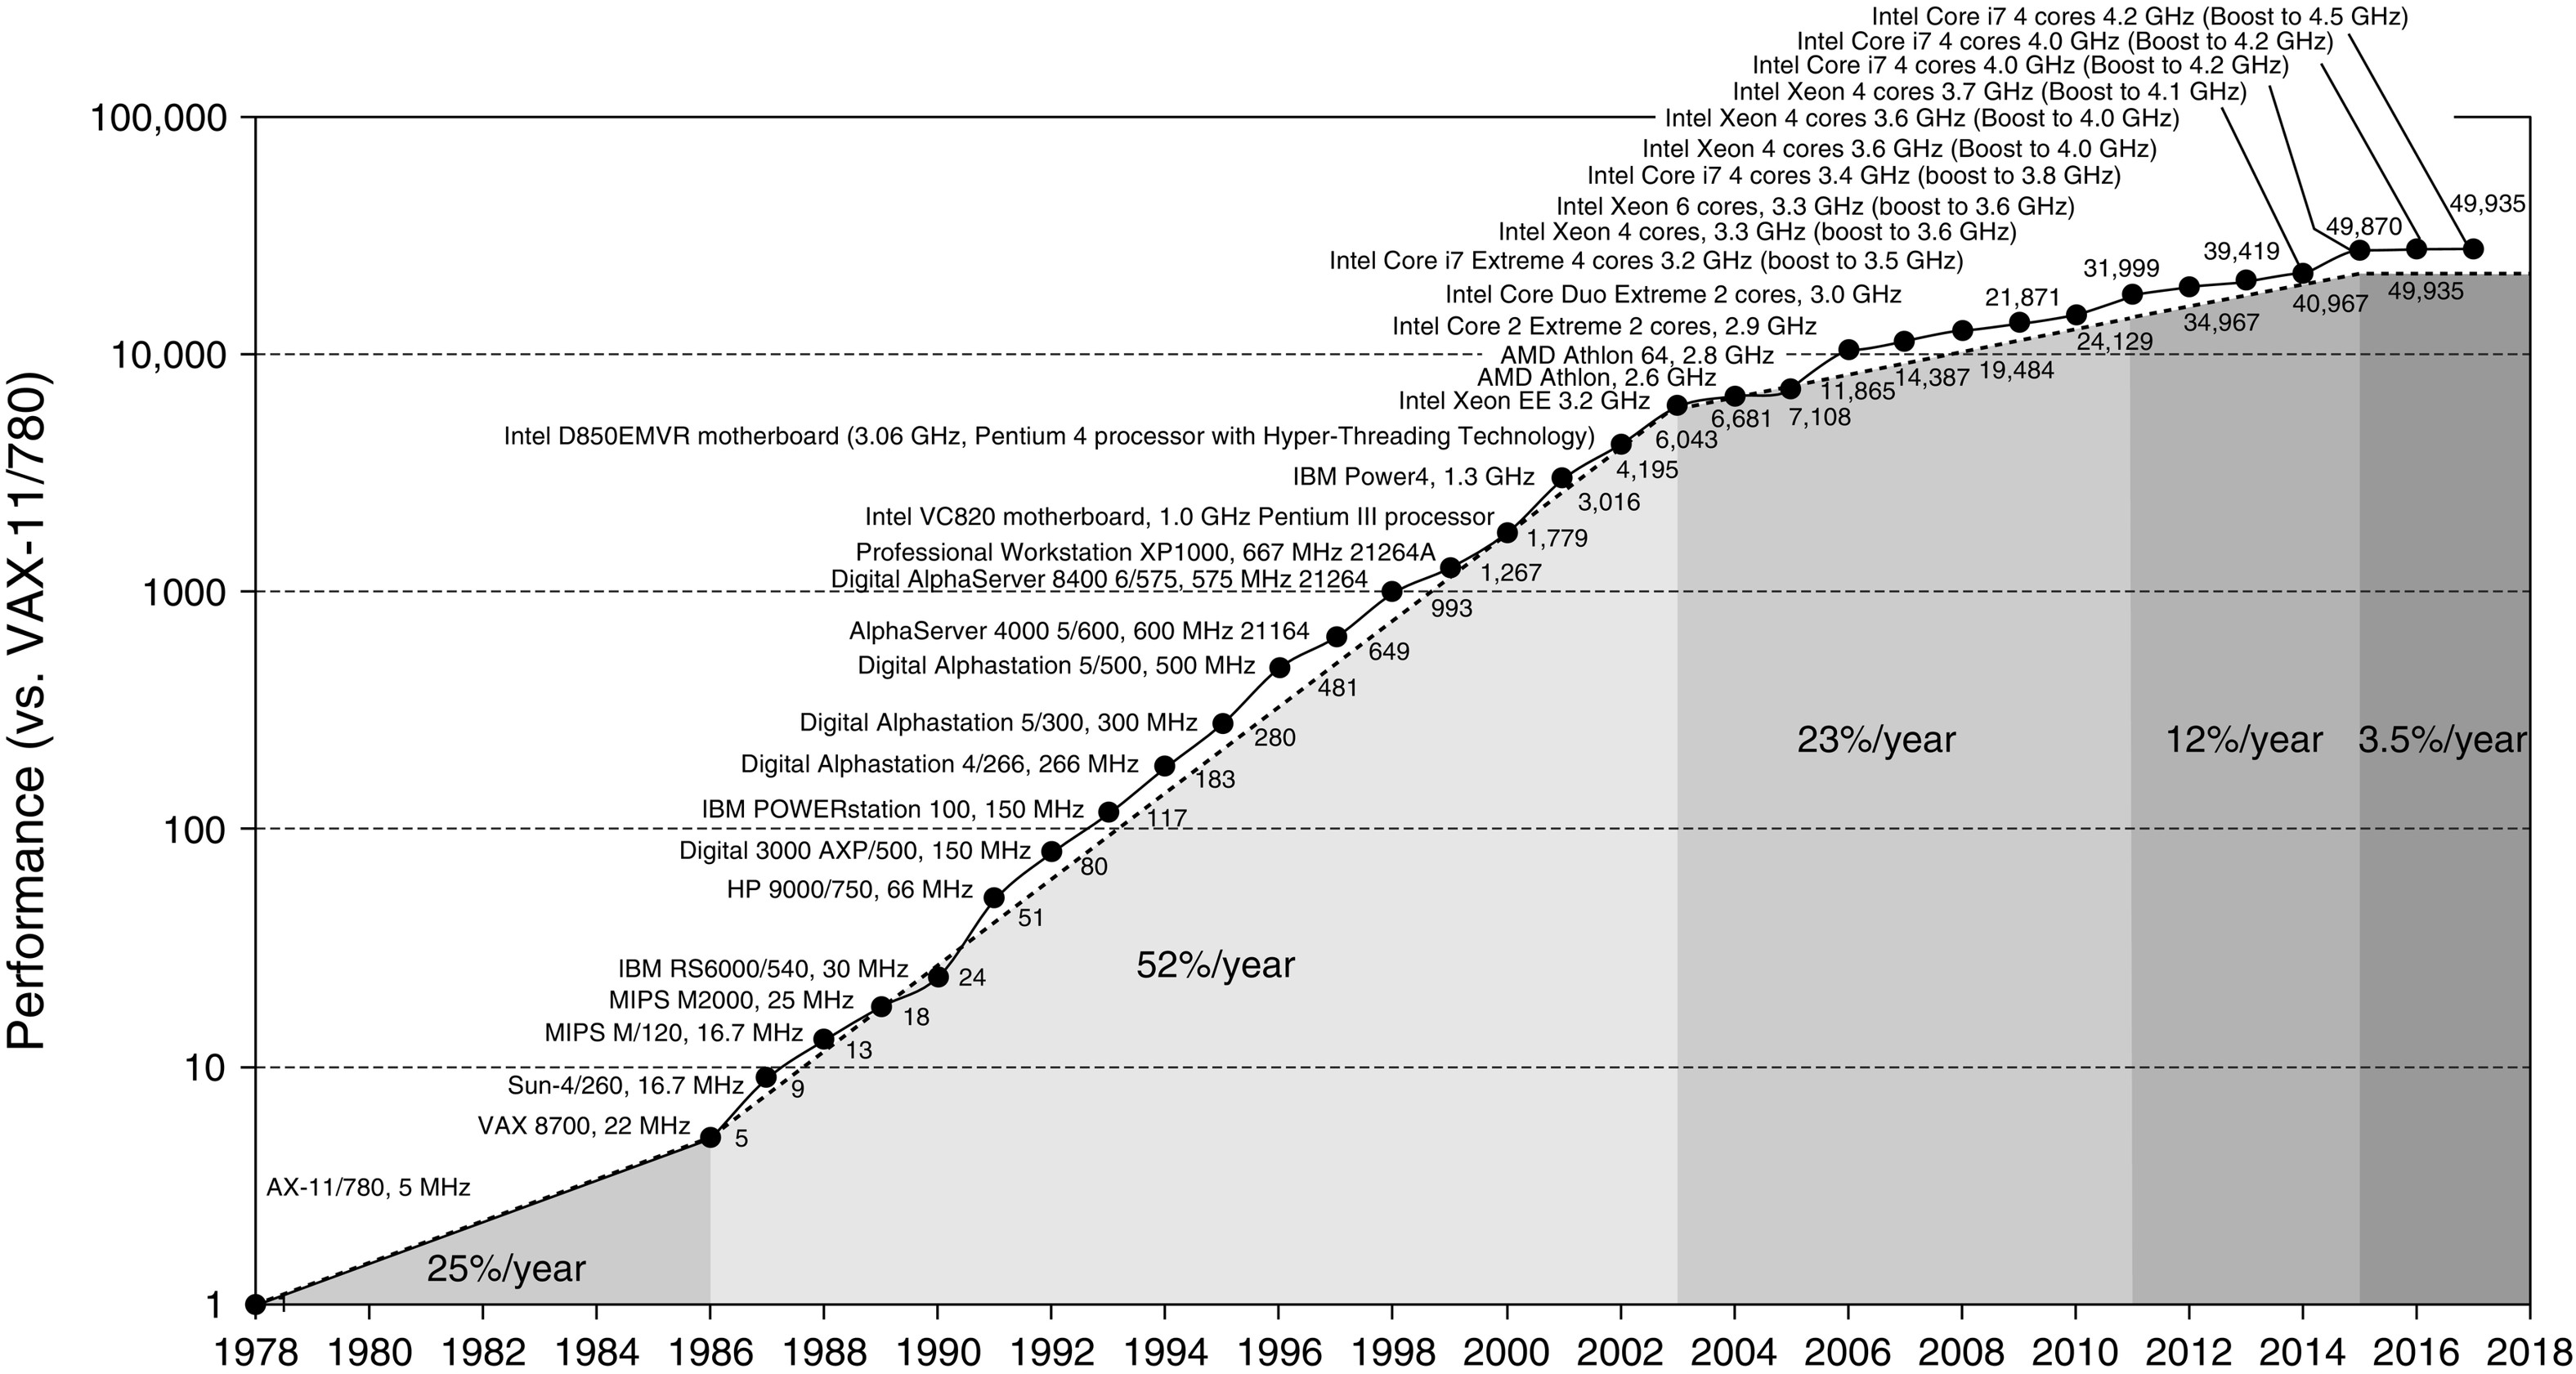
\includegraphics[width=0.8\textwidth]{../Immagini/Capitolo 1/PrestazioniProcessori}
    \caption{Crescita nelle prestazioni dei processori dal 1978 al 2018; il grafico riporta le prestazioni dei processori disponibili sul mercato relative al VAX11/780 misurate attraverso i \textit{benchmark} SPECint.}
    \label{fig:PrestazioniProcessori}
    \par\small{\textit{Fonte: J.L. Hennessy, D.A. Patterson, Computer Architecture: A quantitative Approach. Ed. 6. Waltham, MA:Elsevier, 2017}}
\end{figure}
% Paragrafo 1.3: Le sfide nella progettazione di software parallelo
\section{Le sfide nella progettazione di software parallelo}
\label{par1.3}
Una caratteristica fondamentale posseduta da ogni programma a esecuzione parallela
è la scalabilit\'a, ovvero la capacit\'a di un sistema software di incrementare le proprie prestazioni in funzione della potenza di calcolo richiesta in un preciso istante \cite{Michael2007},
che consente di ottenere architetture tolleranti ai guasti assieme a un'elevata disponibilit\'a del sistema.

% Parte Finale della tesi
% Capitolo 2 (Un linguaggio per il calcolo parallelo: MATLAB)
\chapter{Un linguaggio per il calcolo parallelo: MATLAB}
\label{cap2}
% Introduzione Capitolo 2
L'accesso diffuso a sistemi di elaborazione multiprocessore ha aumentato
la domanda di mercato per soluzioni software a supporto dello sviluppo di programmi a esecuzione parallela. \newline
Gli ambienti di programmazione per il calcolo scientifico, MATLAB (abbreviazione di \textit{Matrix Laboratory}) incluso, hanno recepito questa tendenza,
creando tutte le condizioni necessarie per l'aggiunta di nuove funzionalit\`a dedicate all'elaborazione parallela.

In questo capitolo forniremo una rapida panoramica delle funzionalit\`a di MATLAB per il calcolo parallelo,
con un particolare focus sulle motivazioni e sulle scelte di design che hanno guidato l'implementazione di questa nuova parte del linguaggio.
% Paragrafo 2.1: Gli ingredienti per un MATLAB parallelo
\section{Gli ingredienti per un MATLAB parallelo}
\label{par2.1}
\nocite{Sharma2009}
\subsection{Una breve prospettiva storica}
L'approccio seguito dai progettisti di The MathWorks\footnote{La \textit{software house} statunitense, con sede in Massachusetts (Stati Uniti), che si occupa dello sviluppo di MATLAB e di altri prodotti per il calcolo scientifico.}
per estendere MATLAB  al mondo del calcolo parallelo \`e stato modificare le caratteristiche del linguaggio 
stesso, cominciando dall'aggiunta di \textit{routine} comunemente impiegate nella risoluzione di problemi \textit{embarrassingly parallel}. 

A partire dai primi passi compiuti in questa direzione negli anni Ottanta del secolo scorso da Cleve Moler, l'autore del linguaggio, ci si imbatt\'e
nel fatto che il modello di memoria globale di MATLAB, secondo il quale le variabili definite dall'utente e importate dall'esterno vengono conservate 
in un'area di memoria allocata dalla sessione attiva di MATLAB, era in contrasto con il modello di memoria condivisa impiegato dalla maggioranza dei sistemi 
multiprocessore.

Questa incompatibilit\`a causò dei rallentamenti al progetto di parallelizzazione di MATLAB, ma le pressioni esterne di coloro che auspicavano a un suo completamento erano troppo insistenti per essere ignorate.\newline
La crescente disponibilit\`a di sistemi multiprocessore aveva reso il calcolo parallelo un argomento presente sulla bocca di tutti gli specialisti del 
settore; la comparsa delle prime architetture \textit{multicore} e l'ascesa dei \textit{cluster} Beowulf\footnote{I \textit{cluster} Beowulf sono \textit{cluster} costituiti dall'interconessione di componenti hardware commerciali, ad esempio PC al termine della loro vita utile, mediante una tradizionale rete LAN. } permisero una diffusione massiccia dei sistemi di calcolo ad alte prestazioni, che precedette la \enquote{democratizzazione} dei WSC portata dal \textit{cloud computing}.\newline   
Inoltre, MATLAB era gi\`a allora un ambiente di programmazione affermato all'interno della comunit\`a scientifica e quindi doveva fornire ai propri utenti un prodotto completo e funzionale 
in tutti gli scenari applicativi, inclusi i progetti a elevata intensit\`a computazionale.

Ecco che nel novembre del 2004 vennero rilasciati al pubblico i primi risultati di questo progetto, sotto le vesti di due pacchetti software addizionali (chiamati \textit{toolbox} nel vocabolario tecnico del linguaggio): il Distributed Computing 
Toolbox\textsuperscript{\texttrademark} e il MATLAB Distributed Computing Engine\textsuperscript{\texttrademark}\footnote{I due nomi commerciali sono i corrispettivi degli odierni Parallel 
Computing Toolbox\textsuperscript{\texttrademark} e MATLAB Parallel Server\textsuperscript{\texttrademark}.}.

\subsection{Gli aspetti imprescindibili dell'implementazione}
\label{sec2.1.2}
L'adattamento di MATLAB al calcolo parallelo non fu condotto in modo casuale, bens\'i le aggiunte al linguaggio furono ponderate attentamente a partire dalle informazioni ricavate dai sondaggi condotti nelle fasi preliminari del progetto.\newline
Per questo motivo, il modello di programmazione proposto da MATLAB \`e adatto all'esecuzione di programmi paralleli su sistemi \textit{multicore} e su \textit{cluster} di elaboratori, trattandosi delle architetture di calcolo parallelo pi\`u comuni in ambito industriale.

Di seguito elenchiamo, in ordine decrescente di importanza, gli obiettivi di progettazione che ispirarono e continuano a ispirare il processo di parallelizzazione di MATLAB;
\begin{itemize}
    \item la programmabilit\`a, cio\'e la capacit\`a di creare programmi che soddisfino i requisiti degli utenti e che siano facili da mantenere per gli sviluppatori;
    \item l'esecuzione di codice arbitrario sui sistemi multiprocessore supportati;
    \item l'astrazione da dettagli irrilevanti durante l'implementazione; di conseguenza, lo sviluppatore medio non deve pi\`u preoccuparsi di aspetti quali lo \textit{scheduling} delle \textit{task} e la distribuzione dei dati alle unit\`a di lavoro, in quanto vengono gestiti automaticamente dal linguaggio;
    \item l'indipendenza del programma dall'allocazione delle risorse computazionali: un software parallelo scritto in MATLAB deve funzionare correttamente sia quando eseguito su un sistema multiprocessore che su un sistema monoprocessore, adattando il suo comportamento alle risorse di calcolo disponibili;
    \item l'accesso a costrutti di programmazione di prima classe\footnote{Secondo la classificazione proposta dall'informatico britannico Christopher Strachey \cite{SICP96}, i costrutti di programmazione di prima classe possono essere manipolati liberamente nelle istruzioni del linguaggio; in pratica, devono poter essere passati come parametri attuali durante l'invocazione di una procedura, restituiti come valore di ritorno di una funzione e assegnati a variabili o a strutture dati.}. 
\end{itemize}
Il percorso di trasformazione di MATLAB al fine di renderlo appetibile al calcolo parallelo non \`e ancora giunto al termine. \newline La destinazione finale fissata 
dagli addetti ai lavori \`e la realizzazione del modello di linguaggio ideato dal direttore tecnico di TheMathWorks, Roy Lurie \cite{Lurie2007},
secondo cui gli esperti di dominio inseriscono annotazioni minimali al codice sorgente per esprimere l'intenzione di eseguire il programma 
su pi\`u processori simultaneamente.

% Paragrafo 2.2: Parallel Computing Toolbox
\section{Parallel Computing Toolbox}
\label{par2.2}
\nocite{MathWorksParallelComputing}
Il \textit{Parallel Computing Toolbox}, spesso abbreviato in PCT, permette di risolvere problemi \textit{compute-intesive} e  \textit{data-intensive} sfruttando 
la capacit\`a di calcolo offerta dalle moderne architetture multiprocessore, come i sistemi \textit{multicore} e i \textit{cluster} di elaboratori. \newline
Costrutti di programmazione di alto livello, come i vettori distribuiti, consentono di sviluppare applicazioni MATLAB scalabili senza ricorrere alla programmazione 
MPI \footnote{La \textit{Message Passing Interface}, o semplicemente MPI, rappresenta lo standard per il modello di comunicazione interprocesso, basato sullo scambio 
di messaggi, impiegato nelle elaborazioni parallele su sistemi distribuiti \cite{NMSUMPIIntro}}.\newline
Inoltre, la stessa applicazione pu\`o essere eseguita su \textit{cluster} o su server in \textit{cloud} senza apportare alcuna modifica al codice grazie a MATLAB 
\textit{Parallel Server}, cos\`i da concentrarsi esclusivamente sullo sviluppo dell'algoritmo migliore per il caso d'uso in esame.

Incominciamo il nostro studio del PCT riportando alcune definizioni, tratte dalla documentazione ufficiale di MATLAB \cite{MathWorksWhatIsParallel}, di aspetti del modello di programmazione parallela fondamentali per la prosecuzione della trattazione.
\begin{itemize}
\item \textit{Client}: termine impiegato per identificare la sessione di MATLAB attiva con cui l'utente finale sta interagendo; tipicamente coincide con il 
\textit{computer} usato dallo sviluppatore durante la prototipazione e lo sviluppo in locale del programma a esecuzione parallela.\newline
Attraverso le funzionalit\`a offerte dal PCT, un \textit{client} gestisce la computazione da eseguire suddividendola in  \textit{task} atomiche e assegnando ciascuna 
di esse a un \textit{worker}.
\item \textit{Parallel Pool}: spesso abbreviato in parpool, \`e un insieme di \textit{worker} comunicanti che possono eseguire codice interattivamente.
\item \textit{Worker}: corrisponde a un'istanza di MATLAB, priva di interfaccia grafica, controllata da un \textit{client} e in grado di fornire la potenza del 
motore di calcolo del linguaggio.
\end{itemize}

Una prima distinzione da sottolineare \`e quella tra l'infrastruttura e i componenti del linguaggio esposti dagli strumenti di calcolo parallelo in MATLAB. 
Il linguaggio comprende costrutti di programmazione parallela e funzioni con supporto automatico al parallelismo mentre l'infrastruttura riguarda i meccanismi 
che coaudivano il linguaggio, come il protocollo seguito per il trasferimento del codice e dei dati alle unit\`a di lavoro del sistema. \newline
Nelle prossime sezioni, esamineremo da vicino alcuni costrutti paralleli offerti da MATLAB, ignorando l'infrastruttura sottostante, nonostante entrambe le componenti 
siano imprescindibili per il corretto funzionamento delle funzionalit\`a parallele del linguaggio.

L'architettura di riferimento fino alla fine del capitolo \`e schematizzata in figura \ref{fig:ArchitetturaRiferimento}.\newline
MATLAB \textit{Parallel Server} comprende un insieme di \textit{worker}, in esecuzione sui nodi di un \textit{cluster}, che ricevono le 
\textit{task} computazionali assegnate dal \textit{client} attraverso specifiche funzioni del \textit{Parallel Computing Toolbox}. \newline
I \textit{worker} prelevano il codice da eseguire e i dati su cui lavorare da una memoria di massa condivisa popolata dall'\textit{head node} 
(non rappresentato in figura), un nodo speciale eletto all'interno del \textit{cluster} responsabile della schedulazione delle attivit\`a sul \textit{cluster}.\newline
Una volta terminata l'elaborazione, i risultati vengono raccolti dal nodo \textit{master} e trasferiti all'interno dello spazio di lavoro del \textit{client} 
mediante il canale di comunicazione instaurato tra il \textit{client} e i \textit{worker} di MATLAB \textit{Parallel Server}.

\begin{figure}[htbp]
    \centering
    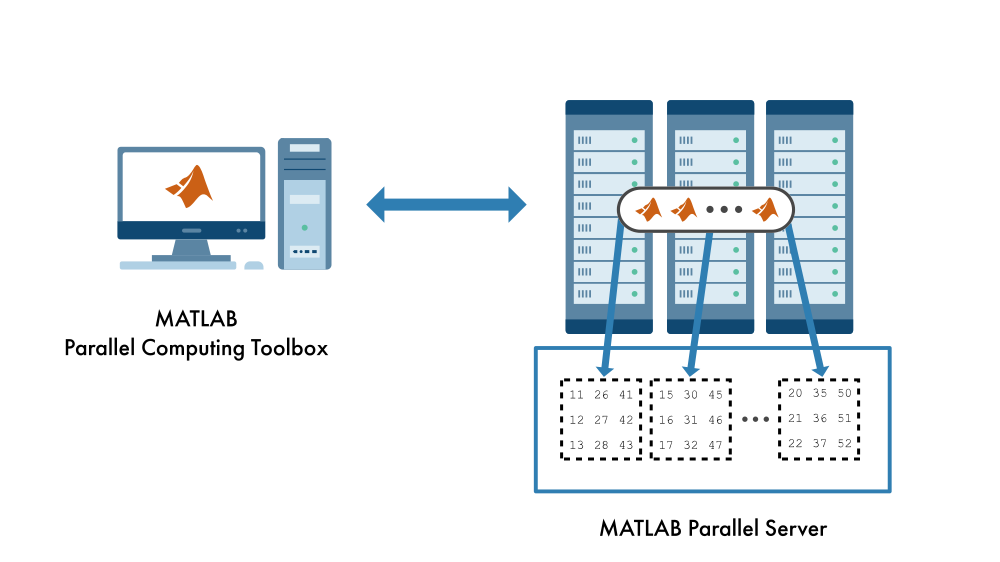
\includegraphics[width=0.8\textwidth]{../Immagini/Capitolo 2/ReferenceArchitecture.png}
    \caption{Architettura di riferimento per gli strumenti di calcolo parallelo in MATLAB. 
    \small{(Da \url{https://it.mathworks.com/products/matlab-parallel-server.html})}}
    \label{fig:ArchitetturaRiferimento}
\end{figure}

Giunti a questo punto, introduciamo le modalit\`a di esecuzione del software parallelo su un sistema multiprocessore supportate dall'ambiente MATLAB:
\begin{itemize}
    \item parallelizzazione implicita: alcune funzioni, se richiamate dal codice sorgente del programma, sfruttano le librerie di \textit{runtime} del linguaggio 
    in modo da essere eseguite su \textit{thread} distinti all'interno della stessa sessione;
    \item parallelizzazione esplicita: il carico di lavoro del programma viene automaticamente suddiviso in \textit{task} elementari, ciascuna delle quali viene 
    poi assegnata a un \textit{worker} per l'esecuzione.
\end{itemize}

\nocite{MathWorksParallelQuickStart}
\subsection{Il paradigma di programmazione parallela implicita}
I \textit{toolbox} di MATLAB sono dotati di un crescente numero di funzioni con supporto automatico al parallelismo, al fine di beneficiare di tutti 
i vantaggi propri dall'elaborazione parallela senza modificare il codice scritto per la versione seriale del programma, in accordo con i principi di design elencati 
nella sezione \ref{sec2.1.2}. 

Alcune funzioni, come \lstinline|mldivide| per la risoluzione di sistemi di equazioni lineari, vengono eseguite automaticamente in parallelo su \textit{thread} 
distinti se invocate dalla sessione principale di MATLAB. 

Ragionando sulla nostra architettura di riferimento, il parallelismo implicito viene attivato solo quando la funzione viene eseguita direttamente dal \textit{client}, 
mentre viene sconsigliato se l'esecuzione \'e a carico dei nodi del \textit{cluster} per evitare un parallelismo \enquote{annidato} che degraderebbe le prestazioni 
dell'intero sistema. \newline
In quest'ottica, possiamo notare come i progettisti del linguaggio abbiano pensato ai \textit{worker} come a unit\`a di elaborazione a singolo \textit{thread}.

Quando il \textit{client} incontra una funzione con supporto automatico al parallelismo nel codice sorgente del programma, avvia un \textit{parallel pool} per la 
sua esecuzione in parallelo. \newline
Un apposito profilo di configurazione determina le caratteristiche dell'ambiente di elaborazione parallela e, in particolare, PCT permette di scegliere tra i 
seguenti profili preimpostati:
\begin{itemize}
    \item \textit{Processes}: i \textit{worker} vengono attivati come processi indipendenti eseguiti dai \textit{core} fisici del calcolatore ospitante la sessione 
    principale di MATLAB.
    \item \textit{Threads}: i \textit{worker} sono eseguiti da \textit{thread} e non pi\`u da processi veri e propri. I vantaggi portati da questo ambiente 
    parallelo sono un minor uso di memoria, un basso costo di comunicazione tra i \textit{worker} e uno \textit{scheduling} delle attivit\`a particolarmente 
    performante, a scapito della disponibilit\`a di una ristretta gamma di funzioni con supporto al parallelismo su \textit{thread}.
\end{itemize}
Relativamente alla scelta del numero di \textit{worker} nell'ambiente \textit{Processes} \'e consigliato riservare un motore di calcolo per ogni \textit{core} 
fisico disponibile, ignorando la presenza di eventuali \textit{core} virtuali; infatti, questi ultimi condividono alcune risorse di calcolo all'interno dello 
stesso processore, tra cui la \textit{Floating Point Unit} (FPU), e poich\'e la maggior parte delle elaborazioni in MATLAB richiede l'esecuzione di operazioni 
aritmetiche in virgola mobile, limitare a uno il numero di \textit{worker} per unit\`a di esecuzione pu\`o aumentare la stabilit\`a del sistema. \newline 
L'unica eccezione \`e rappresentata dalle applicazioni \textit{data-intensive}, per le quali potrebbe essere conveniente portare il numero di \textit{worker} per 
\textit{core} fisico a due.

In ogni caso, un singolo \textit{parpool} a supporto della parallelizzazione implicita pu\`o contenere fino a 512 \textit{worker}, a prescindere dalle specifiche 
del calcolatore utilizzato.
\begin{figure}[htbp]
    \centering
    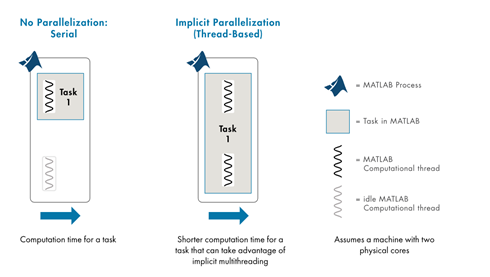
\includegraphics[width=0.8\textwidth]{../Immagini/Capitolo 2/ImplicitParallelization.png}
    \caption{Rappresentazione del modello di parallelizzazione implicita di MATLAB su un sistema \textit{dual-core}
    \small{(Da \url{https://it.mathworks.com/discovery/matlab-multicore.html})}}
    \label{fig:ParallelismoImplicito}
\end{figure}\newline
Se una funzione non include il supporto automatico al parallelimo, possiamo trasferire l'esecuzione del programma a una \textit{workstation}, in modo da beneficiare 
dello \textit{speedup} offerto da un sistema con maggiore capacit\`a di calcolo, oppure possiamo utilizzare il paradigma di programmazione parallela esplicita 
supportato dal \textit{Parallel Computing Toolbox}.

\subsection{Il paradigma di programmazione parallela esplicita}

Il modello di programmazione parallela esplicita esposto dal \textit{Parallel Computing Toolbox} si fonda sull'esistenza di costrutti di programmazione 
parallela a diversi livelli di astrazione, di cui i programmatori si possono avvalere durante la stesura di programmi a esecuzione parallela.\newline
Il meccanismo a bassissimo livello presente per la scrittura di programmi a elaborazione parallela \`e basato sullo scambio di messaggi tra i \textit{worker} 
appertenenti a un medesimo \textit{parallel pool}, ma lo sviluppo di programmi secondo questo approccio viene spesso criticato, essendo considerato l'equivalente del linguaggio 
Assembly per la programmazione parallela.\newline
Per agevolare la scrittura di software parallelo, alcuni costrutti di programmazione di alto livello sono introdotti nel linguaggio, aumentando il livello di 
astrazione del codice scritto e consentendo ai programmatori di scrivere algoritmi paralleli in modo simile alle loro controparti seriali.

Un esempio di costrutto di alto livello per la programmazione parallela \`e incarnato dagli \textit{array} 
\footnote{Nel gergo impiegato da MATLAB, la parola \textit{array} \`e un termine universale per riferirsi a vettori colonna, vettori riga e matrici} 
distribuiti, strutture dati il cui contenuto viene partizionato tra \textit{worker} diversi.\newline
L'impiego di \textit{array} distribuiti permette di memorizzare strutture dati di dimensioni tali da non poter essere contenute nella memoria centrale di un 
singolo calcolatore, sfruttando la capacit\`a di memoria combinata offerta dai nodi del \textit{cluster}.

Gli \textit{array} distribuiti possono contenere dati di qualsiasi tipo e supportano la distribuzione dei loro elementi tra i worker lungo una dimensione, ovvero 
per riga oppure per colonna; a questo proposito, dobbiamo precisare che l'utente ha la possibilit\`a di definire distribuzioni dei dati alternative e che, 
molto spesso, il partizionamento degli elementi tra le unit\`a di lavoro viene modificato implicitamente dall'esecuzione di certe operazioni, 
come \lstinline|gather| una funzione utile a trasferire un \textit{array} distribuito nello spazio di lavoro del \textit{client}.

Un ulteriore vantaggio derivante dall'uso degli \textit{array} distribuiti \`e l'assenza di differenze sintattiche per l'accesso agli elementi rispetto ai 
tradizionali \textit{array}; l'infrastruttura sottostante garantisce in ogni momento una dsitribuzione dei dati idonea all'esecuzione delle operazioni 
richieste dall'utente.\newline
Questa ampia possibilit\`a di manovra lasciata al programmatore potrebbe introdurre consistenti \textit{overhead} di comunicazione tra i \textit{worker}, 
ma sappiamo che la programmabilit\`a rappresenta l'obiettivo di design prioritario nel processo di parallelizzazione di MATLAB, perfino a scapito delle prestazioni.

Centinaia di funzioni MATLAB native, e altrettante presenti nei \textit{toolbox} sviluppate dalla \textit{community}, sono state progettate per adattare il 
loro comportamento alla ricezione di parametri distribuiti in ingresso.\newline
Ad esempio, MATLAB prevede un ampio insieme di funzioni parallele per l'algebra lineare che operano su \textit{array} distribuiti, implementate a partire dalle \textit{routine} definite dalla libreria di algebra lineare numerica ScaLAPACK.
\backmatter

%Bibliografia
%\bibliographystyle{IEEEtrans}
\printbibliography
\addcontentsline{toc}{chapter}{Bibliografia}
%\bibliography{./Bibliografia/Bibliografia.bib}

\end{document}